\section{Dalitz Plot Analysis}

\subsection{Pairwise invariant masses}

Three-body decays contain more kinematic information than a single reconstructed parent mass. The internal phase-space structure can be studied using pairwise invariant masses. For three daughter tracks labelled $K_1$, $K_2$, and $K_3$, the Dalitz variables used in this project are
\begin{align}
  m^2(K_1K_2), \qquad
  m^2(K_2K_3), \qquad
  m^2(K_1K_3).
\end{align}
Only two of these variables are independent for a fixed parent mass, but plotting different pairs is useful for visual inspection and for checking symmetries or structures involving different track orderings.

The pair mass is computed by summing the two daughter four-vectors:
\begin{equation}
  m_{ij}^2 =
  \left(E_i + E_j\right)^2
  -
  \left|\vec{p}_i + \vec{p}_j\right|^2 .
\end{equation}
As in the B-mass reconstruction, each daughter is assigned the kaon mass hypothesis. The resulting squared masses are reported in \gevfour{} to keep the numerical axis scales readable.

\subsection{Dalitz distributions and resonance structure}

A Dalitz plot displays the density of selected events in a two-dimensional plane of pairwise invariant-mass-squared variables. Resonant two-body substructures can appear as bands, while interference and phase-space effects can produce non-uniform densities. In a complete amplitude analysis, these structures would be modelled with coherent sums of resonant and non-resonant amplitudes. The present analysis restricts itself to visualising the distributions.

Figure~\ref{fig:dalitz_12_23} shows the distribution in the $m^2(K_1K_2)$ versus $m^2(K_2K_3)$ plane. The use of a two-dimensional histogram rather than a raw scatter plot makes dense regions easier to read.

\begin{figure}[H]
  \centering
  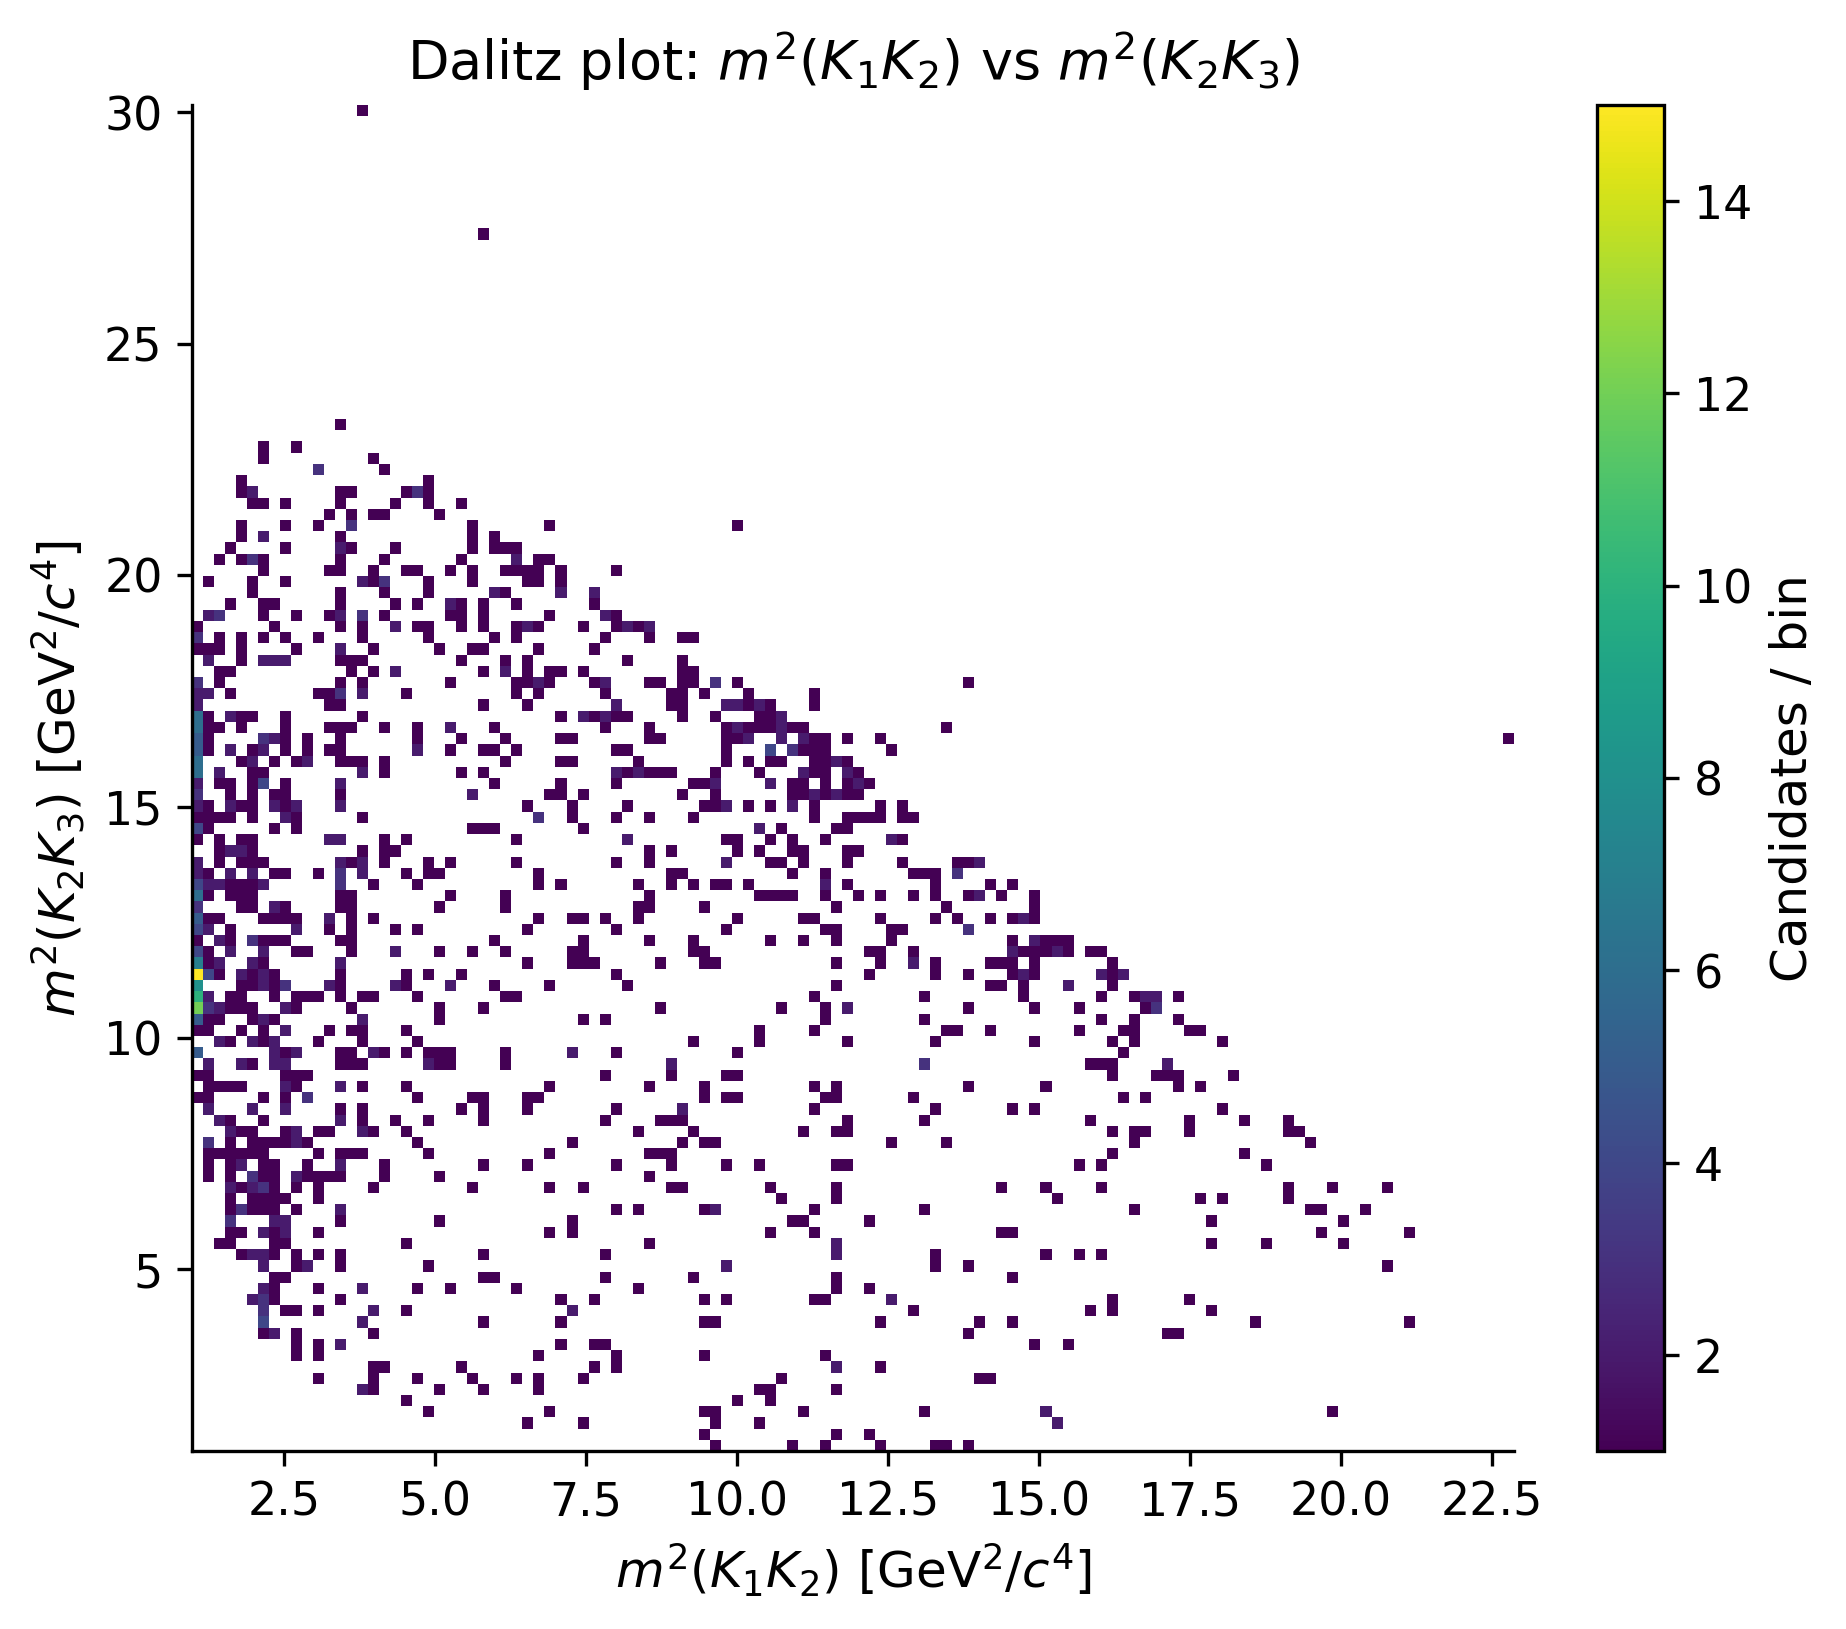
\includegraphics[width=0.78\textwidth]{dalitz_mK1K2_vs_mK2K3.png}
  \caption{Dalitz density map in the $m^2(K_1K_2)$ versus $m^2(K_2K_3)$ plane.}
  \label{fig:dalitz_12_23}
\end{figure}

Figures~\ref{fig:dalitz_12_13} and~\ref{fig:dalitz_23_13} show the complementary pairings. Together, these projections provide a first view of the three-body phase-space population after the baseline selection.

\begin{figure}[H]
  \centering
  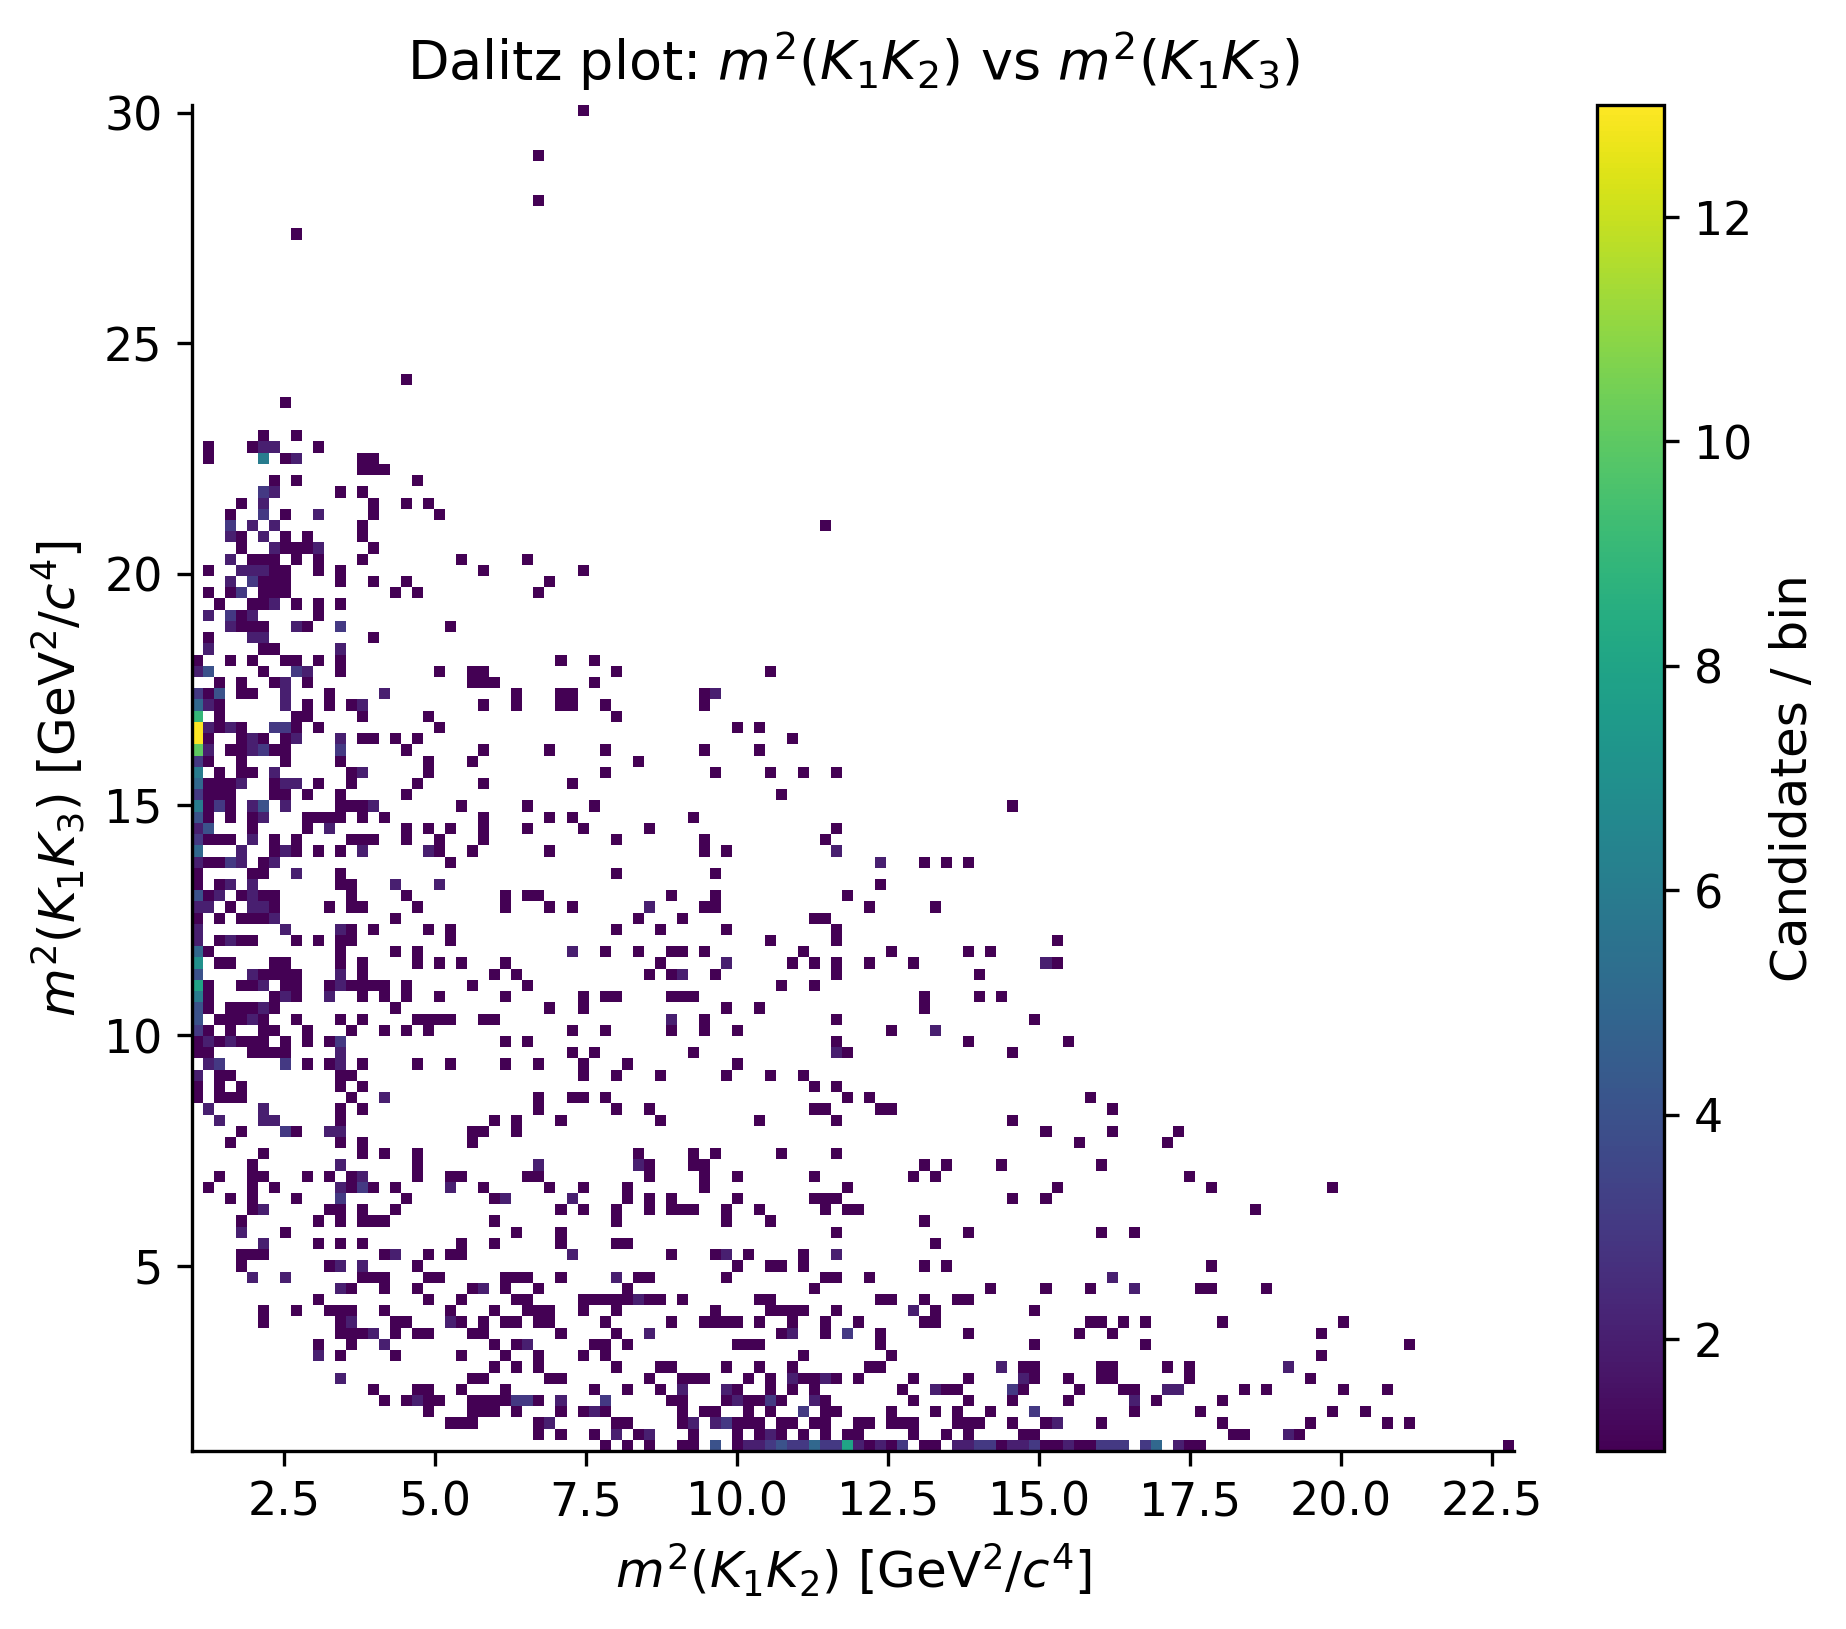
\includegraphics[width=0.78\textwidth]{dalitz_mK1K2_vs_mK1K3.png}
  \caption{Dalitz density map in the $m^2(K_1K_2)$ versus $m^2(K_1K_3)$ plane.}
  \label{fig:dalitz_12_13}
\end{figure}

\begin{figure}[H]
  \centering
  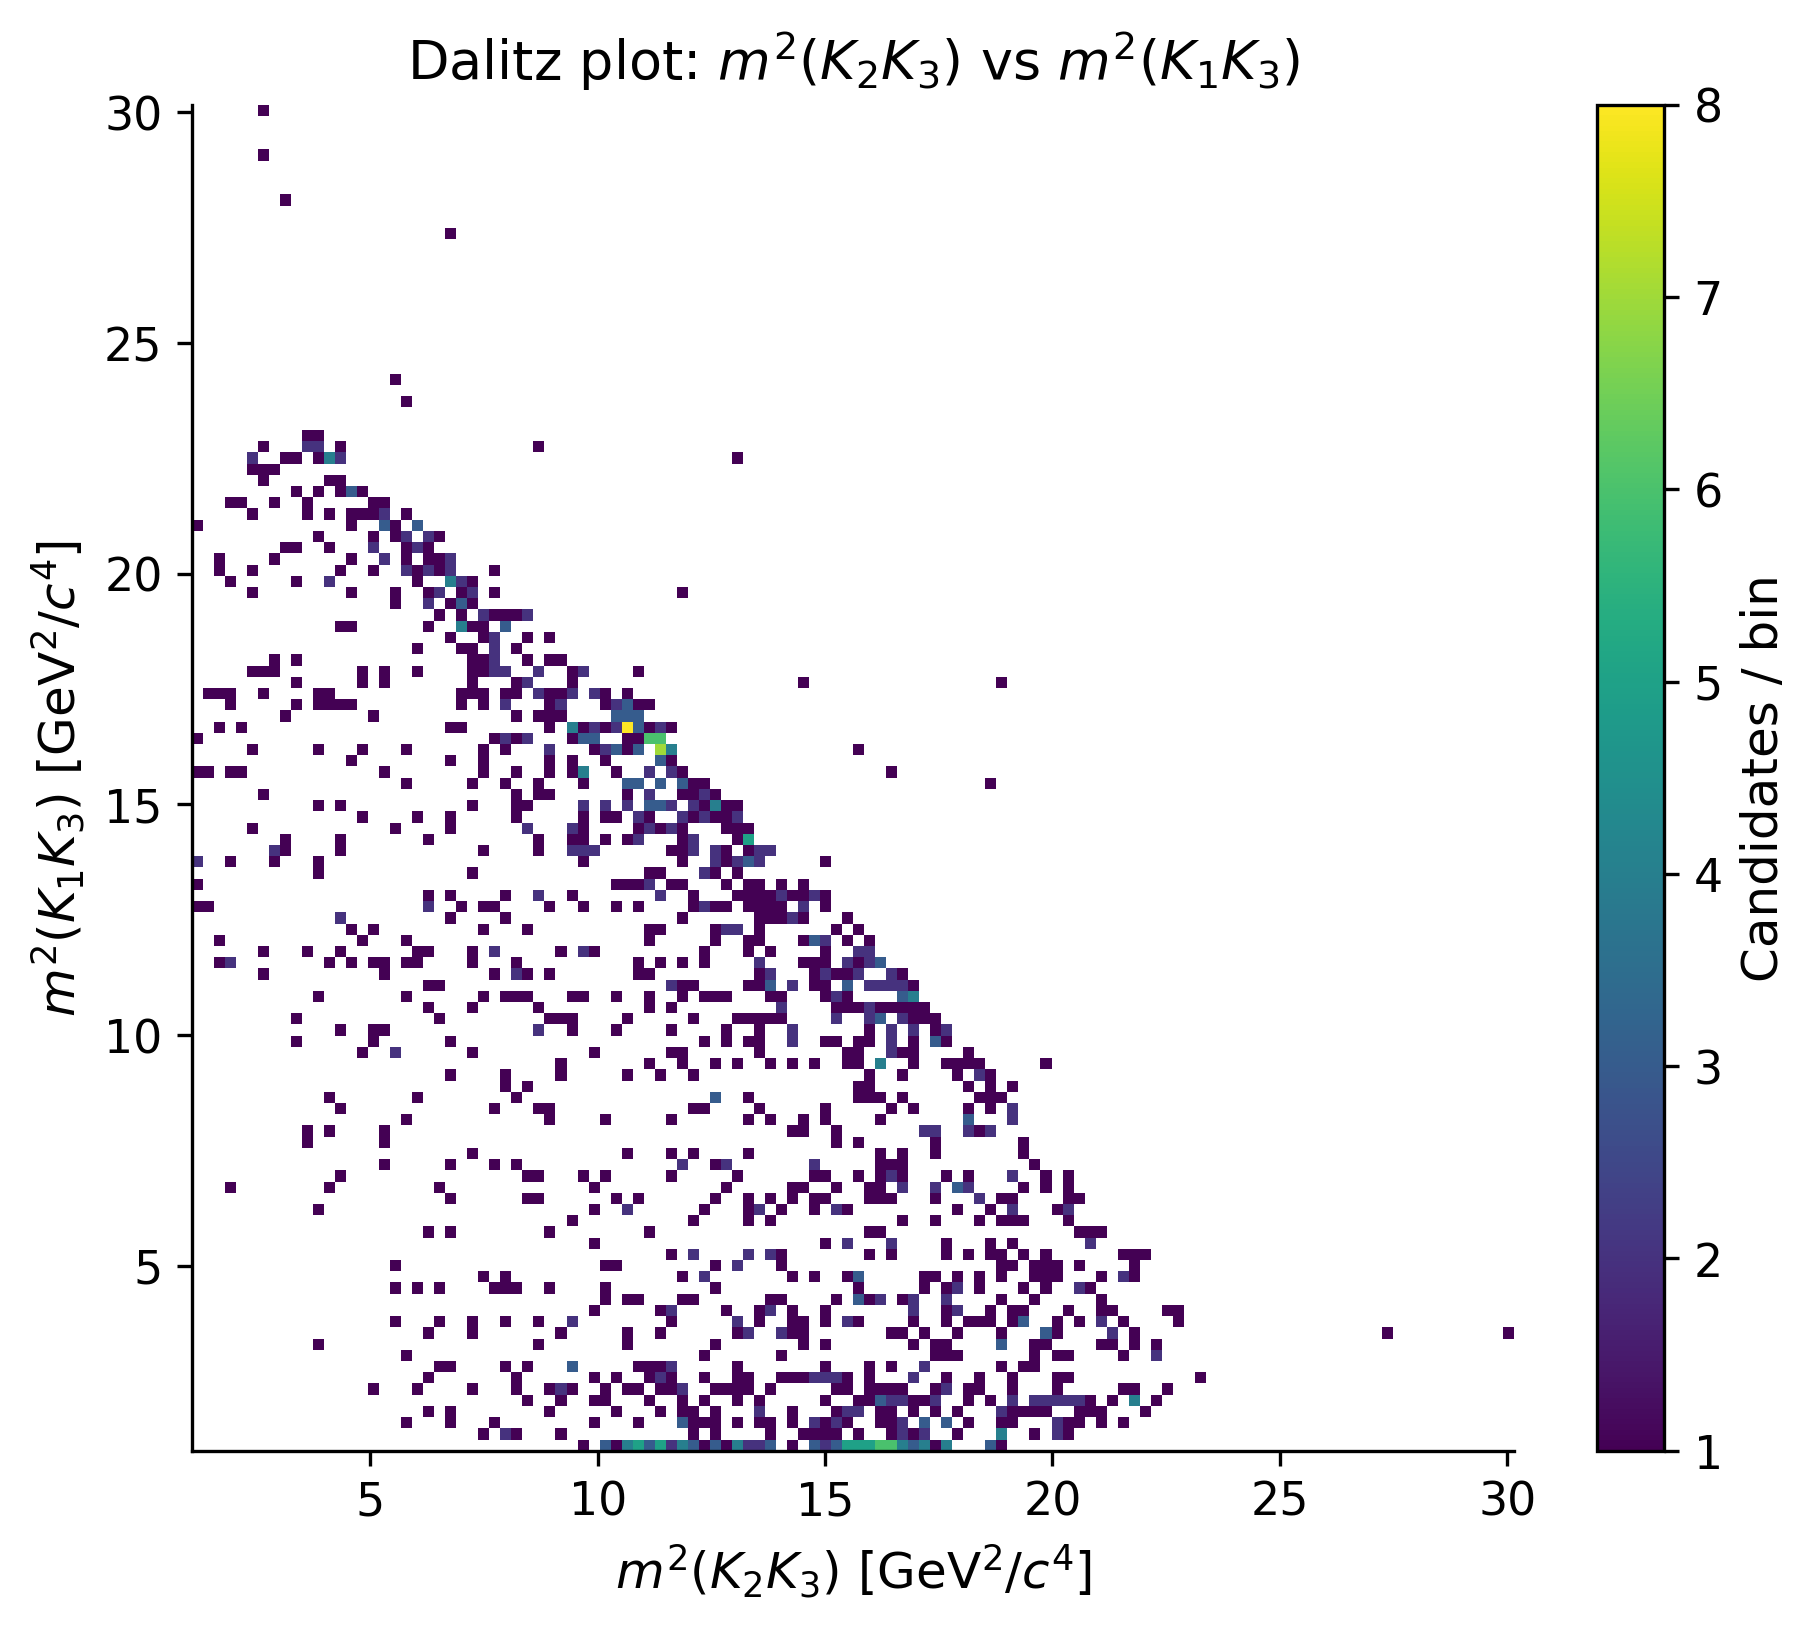
\includegraphics[width=0.78\textwidth]{dalitz_mK2K3_vs_mK1K3.png}
  \caption{Dalitz density map in the $m^2(K_2K_3)$ versus $m^2(K_1K_3)$ plane.}
  \label{fig:dalitz_23_13}
\end{figure}

Dalitz plots are especially relevant for CP-violation studies in multibody decays. Even if the integrated raw asymmetry is small, local asymmetries in restricted phase-space regions can be larger. A natural future extension would therefore compare the Dalitz distributions of \Bplus{} and \Bminus{} candidates, using background subtraction and detector-efficiency corrections.
